
In this chapter we will describe the different parts of the system and how the
identification protocols will work.
%In this section we describe the user identification system. 
%This system provides a distributed and secure way to attain a user-password
%identification scheme like the ones commonly seen in centralized services.

\section{Architectural principles}

\subsection{Securing the nodes of a leafset}

%% Refering to the section in the paper "A Scalable Architecture for Highly Reliable Certification"
The first step to requesting a service is to acquire the set of nodes that
compose the leafset for a given root key $K$. Supposing that $K$ is associated
with node $K_{ROOT}$, there remains a probability for $K_{ROOT}$ to be
malicious. $K_{ROOT}$ might lie and provide references to other malicious nodes
in order to collude against the requester, or it might deny any service by
remaining silent. Therefore, a simple request to $K_{ROOT}$ will not suffice to
acquire a reliable leafset associated with $K$.

So, if the first query to secure the leafset nodes fails, redundancy is needed.
Our solution  for mitigating this issue is to obtain and compare the leafsets
of at least 3 nodes within the leafset of node $K_{ROOT}$.
To obtain the leafsets of a node we use the Diversity routing algorithm
proposed in~\cite{castro2002secure}. Diversity routing sends copies of the message
along diverse routes to the destination nodes, using different
neighbours of the source nodes. To avoid attacks based on locality, it uses a
constrained routing table, allowing only the logically closest nodes to be inserted
in the tables. 
%Redundancy sends multiple copies of the same message in order to improve the probability of success, at the cost of
%higher message overheads.
The diversity of the routing tables on each node guarantees a very high probability
of reaching root node $K_{ROOT}$ using different paths, and therefore of
entering the leafset of $K_{ROOT}$ via different nodes. This makes for a more
secure way of acquiring the leafset associated with a key $K$.



%Diversity routing~\cite{castro2002secure}, multiple redundant router
%algorithm~\cite{wallach2003survey} and
%multiple path routing~\cite{artigas2005novel} are some examples of this type
%of approach. Diversity routing sends copies of the message
%along diverse routes to the destination nodes, using different
%neighbours of the source node~\cite{castro2002secure}.
%The Wallash approach~\cite{wallach2003survey}
%also sends multiple copies to all neighbours of the source nodes.
%To avoid attacks based on locality, it uses a constrained routing
%table, allowing only the logically closest nodes to be inserted
%in the tables. The Cyclone multipath routing approach~\cite{castro2002secure}
%increases the number of disjoint paths among the peers in the
%overlay.


Also, we will be using a solution build over a reputation system to improve the
routing process probability of success. The idea is to ignore the nodes with
bad reputation during the routing and look-up process.
Our approach builds a ring structure so that all honest nodes are
linked together, and can contact each other to deliver a trusted
service.


%Fetodova and Veltri~\cite{fedotova2009reputation} integrate a
%reputation system with the process of routing and data lookup
%for a DHT structure. The idea is to ignore the nodes with
%bad reputation during the routing and look-up process.  Dewanet al.~\cite{dewan2004using} use reputations based on the history of
%nodes relaying packets to ensure a packet will be successfully
%delivered in a mobile ad hoc network. In this case the next
%hop is sent to the choice with the highest reputation value.
%However, the highest reputation value may not be good enough.
%Our approach builds a ring structure so that all honest nodes are
%linked together, and can contact each other to deliver a trusted
%service.

%Huang et al. present RouteGuard~\cite{huang2010routeguard}, a scheme that
%distinguishes between cooperative and uncooperative nodes in
%the routing process. Using a reputation system, the nodes fill
%their routing tables with cooperative nodes, thus isolating the
%uncooperative ones. This approach does not
%allow to find new cooperative nodes. Moreover, this approach
%does not consider the dynamism of peer behaviour, which can
%cause fluctuations of the reputation values.

As the idea of using a reputation system to improve the routing process is not
new, we use as a basis the DiversityTrustedRoute
algorithm~\cite{rosas2011corps}.
It searches for honest nodes to improve the service, and as seen in the
diversity routing before, uses different nodes as starting points in order to
reach the same root node $K_{ROOT}$.

If a node $X$ wants to obtain the leafset of a node $K_{ROOT}$, the node $X$ sends a get\_leafset\_root request.
Each node that receives this request checks in its leafset if the $K_{ROOT}$
node is present. If this condition is met, the node responds with its own
leafset and ends the request.
After the node $X$ receives the first leafset it runs a filter to obtain the
$L/2$ nodes  below $K_{ROOT}$ and the $L/2$ nodes above $K_{ROOT}$. Then
queries directly for the leafset of the farthest filtered node to complete
the missing nodes of the leafset of $K_{ROOT}$.  If the queried node is
malicious and do not respond,  the node $X$ can try querying the next node of
the filtered list.
%%% NOT SURE IS THIS VALIDATION IS DONE OR NOT, does not add much more security
%%% to the protocol, mainly because the nodes can collude and lie altogether
%After the node $X$ recieves the first
%leafset, to avoid having a malicious node lie about the
%leafset sent, the node $X$ validates if the leafset nodes correspond to the leafset of
%the node $K_{ROOT}$ making a query to each one for the key $K$.
%%%

An example of this method is shown in~\ref{fig:secure_routing}. The node $X$
sends a message of the type get\_leafset\_root which reaches the node $K_{-2}$.
Using a value of $L = 4$, the node $K_{-2}$ checks its leafset for the root
node $K$ by doing $K_{-4} \le K \le K_{ROOT}$, and after validating that $K_{ROOT}$
is in its leafset, the node $L_{-2}$ sends his own leafset to the node $X$.
Then the node $X$ filters the received leafset to obtain the set of nodes 
$L = \{K_{-1}, K_{-2}\}$ that are part of the leafset of $K_{ROOT}$,  and
continues to request for the leafset of the node $K_{-1}$. Finally, the node $X$
requests the leafset of the node $K_{1}$ and completes the leafset of the node
$K_{ROOT}$. The worst case is when the $K_{ROOT}$ node is malicious and the
get\_leafset\_root request reaches the farthest node in its leafset. In that
case, the filtering function returns only $L/2$nodes. Is all $L/2$ nodes in the
leafset are malicious, the node $X$ fails to recover the leafset. Still, having $L/2$
malicious nodes, with $p$ being the probability of a node being malicious, is
$p^{\frac{L}{2}}$, which is very low for modest values of $L$. Further
analysis of the algorithm probability of failure can be found in~\ref{sec:eval_leafset}.


\begin{figure}[!htb]
\centering
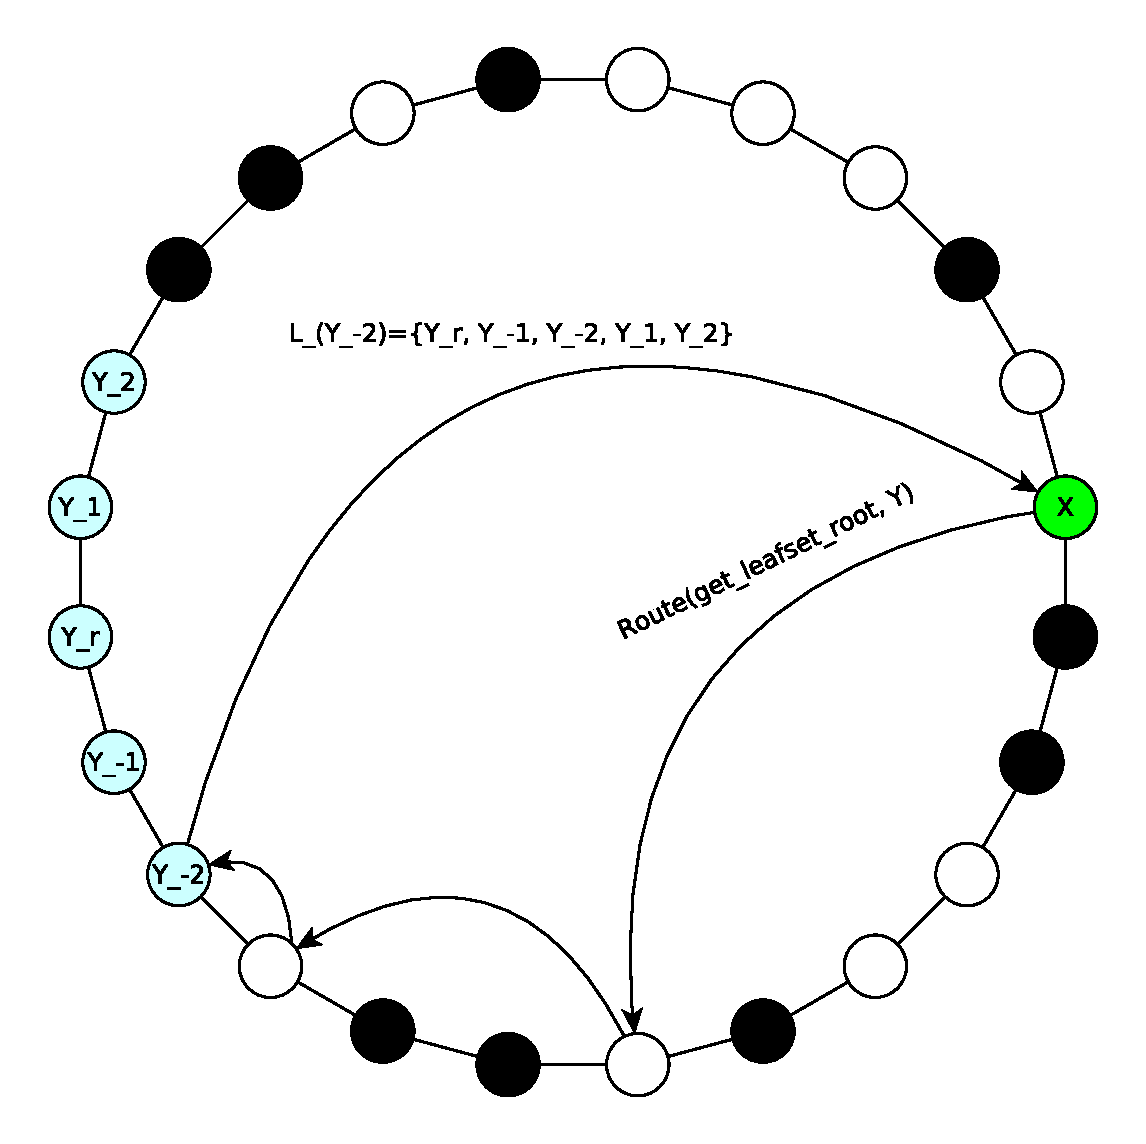
\includegraphics[width=14cm]{../img/secure_routing}\\
\caption{Node $X$ asking for the leafset of the key $K$ using only trusted nodes}
\label{fig:secure_routing}
\end{figure}


\subsection{Normal service request}

Based on the services seen on~\cite{p2p_certification}, to find the nodes associated with a given
service, node $A$ computes the hash
of the service name: $K_s = SHA(ServiceName)$. Let $S_{root} $ be the node that
is closest to $K_s$ in the DHT. $A$ uses DiversityTrustedRoute to acquire the
leafset of $S_{root}$. $A$ thus obtains access to the set $S$ of nodes that
process requests for service $ServiceName$. Let $L$ be the number of nodes in a
leafset: $card(S) = L + 1$.

Once $A$ has acquired $S$, it proceeds to the inception of its service request
by sending a $RequestInit$ message to every node in $S$. A $RequestInit$
message contains a public key $A^{pub}$ of client $A$. In reply to such a
message, every node $S_i$ sends its own public key $S^{pub}_i$. In order to
avoid man-in-the-middle attack, all the ensuing communications between $A$ and
nodes that belong to $S$ will use a public/private key encryption scheme to
ensure that no other node can read the content of the messages.
% later the node will use his user private key & public key in this exchange

If $A$ receives at least $\frac{L}{2} + 1$ answers from the nodes in $S$, then
$A$ considers that the transaction will proceed. Since $S$ is composed of
common nodes from the DHT, it is possible for some of these nodes to be
malicious. However, as explained in our evaluation of the quasi identification
protocol~\ref{sec:evaluation}, a situation where $S$ contains more than
$\frac{L}{2}$ malicious nodes is highly improbable.

A combination of network failures and/or malicious nodes that choose to remain
silent may prevent $A$ from receiving at least $\frac{L}{2} + 1$ answers. Since
$S$ retains the properties of Pastry's leafset, the numerical closeness of its
nodes in the DHT implies that they will very likely be geographically far on
the Internet. Therefore, the probability of $\frac{L}{2} + 1 $ simultaneous IP
routing failures or node failures, that is the probability for more than
$\frac{L}{2}$ answers to not reach $A$, is very close to zero. To account for
this type of situation, $A$ aborts the transaction if it has not received a
sufficient amount of identical answers after a timeout $\delta t$. this is a
very rare and highly improbable case, as shown by our evaluation
in~\ref{sec:evaluation}.


\subsection{Challenges and computational puzzles}
\label{sec:challenges_puzzles}
A challenge or computational puzzle involve a node $X$ posing a challenge to
$A$ that requires a large amount of computation to solve, but is easy to verify
by the node $X$ that sent the challenge. The idea behind the use of
computational puzzles is to restrict the abuse of certain operations in the
system, making them costly enough to make an attack unfeasible under normal
circumstances, but computationally affordable for normal operations of a node
in the system. As an example, in Borisov et al.~\cite{borisov2006computational} described a
fully decentralized mechanism based on computational puzzles for structured P2P
overlays.


This solutions rises the computational cost of the transaction in a
considerable amount.

%%%% TODO Translate to english

%A pesar de que el usar un puzzzle computacional en una trasanccion hace que el
%costo de esta aumente considerablemente, este debe implementarse de tal forma
%que no sea un inconveniente para un usuario comun de la plataforma. Para esto,
%se puede manejar de que el costo computacional aumente exponencialmente por
%cada consulta adicional que se desee realizar por sobre lo que un usuario
%normal realizaria. Asi, se logra que el costo para un usuario normal sea lo
%suficientemente bajo como para ser imperceptible, mientras que si un usuario
%malintencionado decide abusar del sistema realizando consultas reiteradas al
%mismo se encontrara con un costo incremental como para que no le salga a
%cuenta.

%%%%%%% english translation

Although using a computational puzzle in a transaction makes the cost of this
increase significantly, this can be implemented in a way that does not hinders
or restrains a common user of the system.
By increasing exponentially the cost with each additional
query above what a normal user would conduct, we can manipulate the computational cost that is needed for each
transaction and make them costly enough to discourage an attacker.

%, depending of the number of transactions that the user wants to do
%with the system. 
 %So, it makes the cost for a
%normal user is sufficiently low as to be imperceptible, while if an attacker
%decides to abuse the system by performing the same queries repeatedly found an
%incremental cost as to not leave you account.


%%%%%%%%%%%%%%%%%%%%%


 The following system only needs a challenge that fulfill the
criteria of a computational puzzle, so any kind of puzzle that fits can be chosen for
that purpose.

In~\ref{fig:challenge} we show an example of a challenge being issued by a
service $S$ to a node $A$.

\begin{figure}[!htb]
\centering
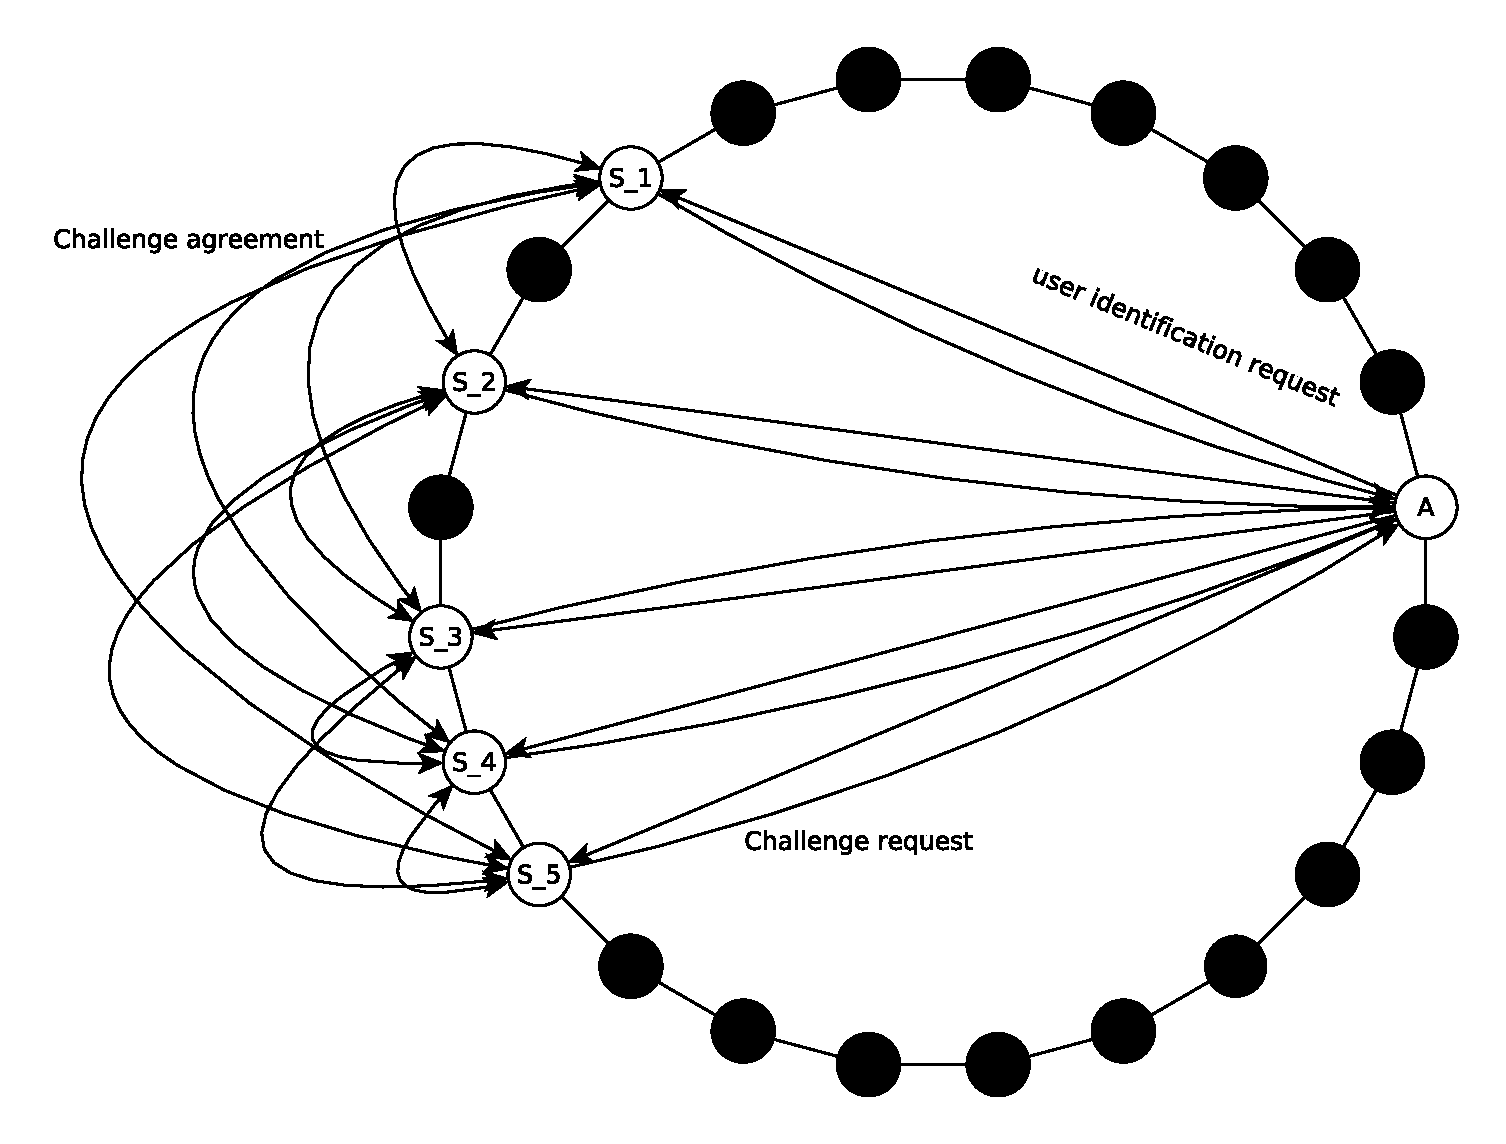
\includegraphics[width=14cm]{../img/challenge}\\
\caption{Service $S$ issuing a  challenge to node $A$}
\label{fig:challenge}
\end{figure}

\subsection{User identification service}
\label{sec:identificators}
%%% more message costly version:
%%A set of $N$ nodes $I_1, I_2, \cdots, I_{N}$ manage the user information
%%needed for his identification.
%%The node ID of the identificator $i$ of the user $U$ with username $username$ is
%%obtained by the function $I_i = SHA^{i}(username)$.
%%The identificators $I_i$ of the username $username$ forms the identification service $I$ for the user with username $username$.
%%Each identificator $I_i$ administers a number of $L$ replicas of the user information. In Pastry,
%%the replicas are stored in the leafset of each node, while in Chord the $r$
%%successors of each node are used.

Every user registered has a set $I$ of nodes that
will constitute the quasi-secure identification authority for the
identification service.
To determine which  nodes belong to $I$, a node computes its key $K$ such that
$K = SHA(U^{username} \bigoplus SHA(U^{username}))$. 

$I_{root}$ is the node closest to $K$ in the DHT, and the quasi-secure identification authority $I =
{I_1, I_2, \cdots, I_{L+1}}$ for the identification of the user with the
username $username$ is composed of $I_{root}$ and of its leafset secured
through DiversityTrustedRoute. These nodes are called \textit{identificators} of the
user $U$ with username $username$.

 In order to prevent man-in-the-middle attack, we use an asymmetric key
encryption scheme for the communications between a node $A$ and $I$. This
induces that every node in $I$ must exchange public keys with every node that
makes a request for the user information. The initial cost expressed in number
of messages is $2(L+1)$, but this exchange only occurs the first time a
node $A$ requests the user identification service from $I$, as the node $A$
maintains a local cache with the public keys of the nodes $I_i \in I$. Also,
every node $I_i \in I$ maintains a local cache with the public keys of ${I_1,
I_2, \cdots, I_{L+1}}$, and key exchanges only occur again if a new node
replaces one of the original nodes from $I$.

%%%%%%% ---- OLD, NOT APPLICABLE TODAY ----
%%%The general view of the system consists in a multi-layered network based in trusted rings.
%%The general view of the system consists in a double-layered network; a Trusted
%%ring of nodes nested inside a normal DHT, with multiple routing policies
%%depending in the protocol of differents services. The user registration,
%%sign-in, logout and password change operations respectively allow a node to
%%register an user identity, to identify himself with an existing user identity,
%%to remove your user session and to change the password used to sign-in.
%%
%%The system needs to have a \textit{trusted ring} maintained by periodical
%%checks of capacity of his members to remain in the trusted ring and a
%%reputation system to evaluate this. Also, similar to the
%%leafset concept in Pastry, each trusted node needs to maintain a
%%\textit{trustset}, which basically consist in D numerically closest trusted
%%nodes with D/2 clockwise nodes, and D/2 counter-clockwise ones.
%%
%%The system used to build the trusted node infraestructure in the P2P networks
%%needs to regularly asses the ability of the nodes to be part of the trusted
%%ring.
%%
%%The figure shows a basic structure of the system. There are normal nodes and
%%trusted nodes. Every trusted nodes maintains a \textit{trustsets}.

\subsection{Storage service maintenance}
\label{sec:lazy_node_maintenance}

%It is important for the system maintains up-to-date the latest 

As insertions and departures of nodes in the DHT cause modifications of the
leafset, the system needs to update the information stored in the
\textit{identificators} nodes. This can lead to performance degradation and inconsistencies in the
system. If left alone, there can be times where the systems
fails to provide all the nodes $I_i$ needed for the identification authority
$I$.

 %We can minimize the risk of this happening using an maintenance scheme for the identificators nodes data.

 %They can be different types of maintenance approaches: \textit{active}, \textit{lazy} and \textit{opportunistic}.

\paragraph{Active Maintenance}
  In \textit{active maintenance}, a
node handles the failure or departure of an existing node in $I$ (or a new
joining node added to $I$) by sending a copy of its stored user's
information data to the others nodes in $I$.
The user's information consists in the user's public keys. This has to be done on every node in the identification service
%The user's information consists in the user's public keys and salt. This has to be done on every node in the identification service
$I$, with $card(I) = L+1$, being $L+1$ the size of the $I_{root}$ node leafset.

 This algorithm converges quickly, but each times it uses $O((L+1)^2)$ messages
for a quasi-identification authority of $L+1$ nodes.
%% What does pastry do?
Pastry uses a more complex variant of active maintenance that is
bandwidth efficient.
Active maintenance runs the risk of creating a positive feedback cycle as
follows: Consider the case whereby a node's access link to the network is
sufficiently connected, which causes timeouts for the node to believe that one
of its leafset nodes has failed (or left the system). If the peer is recovering
in an active mode, maintenance operations will begin. This operation will add
even more packets to its existing congested network link, which will increase
the likelihood that more other peers will mistakenly deduce that other of its leafset
nodes has failed in the system. As this process continues, congestion collapse
on its access link may eventually happen.
Under low peer churn (rate of which number of nodes are moving in and out of the
system in a specific period of time), active maintenance is efficient and scalable because
maintenance messages are only sent in response to actual overlay membership
change events. As the churn rate increases, however, this process becomes more
expensive. A peer sees more churn when its leafset gets larger in size.

For the distributed storage service, any implementation that maintains an
active maitenance for their storage and provides a write and read operation on
it has the capabilities needed to support our identification system. For
example, PAST~\cite{druschel2001past} is a large-scale persistent p2p storage
utility build in Pastry that can be used to provide storage for our system
protocols.

(.... section in development .....)

% pastry
% pastry basicamente usa mantenimiento activo, agregando un metodo para provar
% si un nodo se ha ido o falla antes de sacarlo de la lista de nodos del
%leafset. para evitar sacar un nodo que se encuentra vivo del set, la consulta
%para comprobar si esta respondiendo se realiza varias veces, utilizando grandes
%tiempos de timeout.
% de la misma forma, no agrega un nodo nuevo si este no ha respondido
% previamente
% en el peor caso aumenta la cantidad de mensajes en (k(L+1)(L)), donde k es la cantidad de
% pruebas que se envian para verificar si un nodo esta vivo o no.

%\paragraph{Opportunistic Maintenance}
%
%In opportunistic maintenance, an identificator node periodically shares its user information
%data set with each of the members in $I$, which responds in kind with its own
%user information data set. This process takes place independently of the peer
%detecting changes in the $I$ set of nodes. A node picks one random member of
%its $I$ set to share .....

%\paragraph{Lazy Maintenance}
%
%%Si esto no se trata, pueden haber momentos en que el sistema falla en obtener
%%todos los nodos de la autoridad de identifacion  $I$.
%
%%each time a node leaves or enters the DHT, the system needs to update the
%%information of the User Identification Service.
%%As nodes entering/leaving the leafset of the DHT leads to inconsistency of the
%%information of the User Identification Service stored in each one,
%
%%Insertions and departures of nodes in the DHT cause modifications of the
%%leafsets, and it is therefore crucial to maintain the consistency of the user's
%%information $S_{username}$ used for his identification procedures. The user's information
%%consists in the user's public keys and salt. This has to be done on every node in the identification service
%%$I$.\\
%
%Upon entering a leafset, a node $X$ must update its own view of the user's
%information. Analog to the lazy log consistency maintenance procedure seen
%in~\cite{p2p_certification}, it starts by following the steps below to find
%which user's information store must be updated.\\
%
%\textit{Step 1:} $X$ constructs the set of nodes
%$N = \{ X_{-L/2}, X_{-L/2 +1}, \cdots, X, \cdots X_{L/2 -1}, X_{L/2} $
%composed of its leafset, and of the $\frac{L}{2} +1$ nodes both on the right
%side and on the left of its leafset. 
%%% TODO: figure example  of this
%In order to build this set of nodes, $X$ can ask the farthest nodes $X_{-L/2}$
%and $X_{L/2}$ of its leafset for their own respective leafsets. If one of these
%nodes fails to answer in a timely manner, $X$ can ask the second to farthest
%node, and so on until its immediate neighbors in the leafset. Having
%$\frac{L}{2} +1$ malicious neighbors on both sides is highly improbable, and
%practically unfeasible: for more details about this statement, please refer to
%our probabilistic evaluation in section~\eqref{sec:eval_lazy_maintenance}. \\
%
%\textit{Step 2:} $X$ computes interval $L$ such that
%$$
%L = [ X_{-L/2} - \frac{| X_{-L/2} - X_{-L/2 +1} |}{2}, X_{L/2} +\frac{|
%X_{L/2} - X_{L/2 -1} |}{2} ]
%$$
%
%
%and sends it to every node in set $N$. Upon reception of this message, every
%node replies with a set of all the usernames $U^{username} \in L$ it
%stores, along with the last information regarding the user's
%information corresponding to each username. Thus the format of a response is a
%variable-size set of pairs $\{ U^{username}, S_{username}\}$.\\
%
%
%\textit{Step 3:} $X$ builds set 
%$Y =  \{ \{U^{username_i}, S_{username_i}\},\cdots,\{ U^{username_j},
%S_{username_j}\} \} $ the union of all received usernames and user's
%information. $X$ then discards all pairs $\{ U^{username}, S_{username}\}$ that
%appear less than $\frac{L}{2} +1$ times in $Y$, since these may have been
%generated by colluding nodes. Once this is done, $X$ synchronizes all the
%user's information store whose username matches one of the remaining usernames
%in set $Y$.\\
%
%% checkpoints -> not used in this implementation
%%For every file of user information that $X$ must synchronize, $X$ selects a node $Z$ in $N$ that
%%holds this user information. If $X$ does not have any entry for this username,
%%then $X$ must ask $Z$ for the entire user's information store. Otherwise, $X$
%%sends the last $q$ public keys and salts it has of the user.
%
%It is essential for $X$ to handle the synchronization as an atomic operation,
%as responding to a change password request while the user information is not up
%to date may lead to problems in further requests. Therefore, $X$ postpones all
%transactions about the user information until the synchronization is over.
%
%\subsection{Node failures and node departures}
%\label{sec:node_failures_and_departures}
%Two situations call for the removal of a node. A normal departure corresponds
%to an honest node that notifies its departure to the nodes of its leafset. In a
%crash departure situation, the node fails silently. Pastry exchanges
%periodical heartbeats among nodes in the same leafset in order to detect such
%failures.\\
%
%Upon removal of a peer in its leafset, a node $X$ will look for a replacement.
%$X$ starts by identifying which side of its leafset it must fix: the left side
%or the right side, depending on the nodeId of the node that was removed. Let $N
%= {N_{\alpha}, N_{\beta}, \cdots, N_{\omega}}$ be the set of $\frac{L}{2} - 1$
%nodes corresponding to the side of the leafset in need of fixing. In order to
%find the next node to add to its leafset, $X$ request the leafset of the
%farthest node $N_{\omega}$ in set $N$. Upon reception of the answer, $X$ then
%inserts in its own leafset the reference to the node closest to $N_{\omega}$
%that does not yet belong to $N$. If $N_{\omega}$ remains silent, $X$ must
%repeat the operation with the second to farthest node in $N$, and so on until
%reaching node $N_{\alpha}$ if no timely answer ever comes back. If $X$ fails to
%receive any answer from the nodes in its leafset, then it cannot repair its
%leafset.\\
%
%Once it has successfully fixed its leafset, $X$ must synchronize its user's
%information. $X$
%uses DiversityTrustedRoute to acquire the leafset of the node it has just
%added. $X$ then synchronizes its stored user's information with the nodes in
%the acquired leafset by means of the scheme described in~\ref{sec:lazy_node_maintenance}.
%
%%%\subsection{Active user information store maintenance}
%%%\label{sec:active_node_maintenance}
%%%
%%%%Insertions and departures of nodes in the DHT cause modifications of the
%%%%leafsets, and it is therefore crucial to maintain the consistency of the user's
%%%%information $S_{username}$ used for his identification procedures. The user's information
%%%%consists in the user's public keys and salt. This has to be done on every node in the identification service
%%%%$I$.\\
%%%
%%%There can be a successful operation that involved only $L+1/2$ nodes. That means
%%%that almost half of the nodes in charge had some kind of problem during the
%%%operation proccess. With a lazy store maitenance, there can be a large amount
%%%of time where the nodes will not be synchronized, so an active store maitenance
%%%is needed.
%%%
%%%Upon a successfully user registration or password change operation,
%%%%To propagate changes in the user information to every node in charge,
%%%every node that participated in the operation sends a
%%%message to every node in his leafset notifying about the changes incurred. If a
%%%node ........
%%%
%%%
%%%Upon entering a leafset, a node $X$ must update its own view of the user's
%%%information. Analog to the lazy log consistency maintenance procedure seen
%%%in~\cite{p2p_certification}, it starts by following the steps below to find
%%%which user's information store must be updated.\\
%%%
%%%\textit{Step 1:} $X$ constructs the set of nodes
%%%$N = \{ X_{-L/2}, X_{-L/2 +1}, \cdots, X, \cdots X_{L/2 -1}, X_{L/2} $
%%%composed of its leafset, and of the $\frac{L}{2} +1$ nodes both on the right
%%%side and on the left of its leafset. 
%%%%% TODO: figure example  of this
%%%In order to build this set of nodes, $X$ can ask the farthest nodes $X_{-L/2}$
%%%and $X_{L/2}$ of its leafset for their own respective leafsets. If one of these
%%%nodes fails to answer in a timely manner, $X$ can ask the second to farthest
%%%node, and so on until its immediate neighbors in the leafset. Having
%%%$\frac{L}{2} +1$ malicious neighbors on both sides is highly improbable, and
%%%practically unfeasible: for more details about this statement, please refer to
%%%our probabilistic evaluation in section~\eqref{sec:eval_lazy_maintenance}. \\
%%%
%%%\textit{Step 2:} $X$ computes interval $L$ such that
%%%$$
%%%L = [ X_{-L/2} - \frac{| X_{-L/2} - X_{-L/2 +1} |}{2}, X_{L/2} +\frac{|
%%%X_{L/2} - X_{L/2 -1} |}{2} ]
%%%$$
%%%
%%%
%%%and sends it to every node in set $N$. Upon reception of this message, every
%%%node replies with a set of all the usernames $U^{username} \in L$ it
%%%stores, along with the last information regarding the user's
%%%information corresponding to each username. Thus the format of a response is a
%%%variable-size set of pairs $\{ U^{username}, S_{username}\}$.\\
%%%
%%%
%%%\textit{Step 3:} $X$ builds set 
%%%$Y =  \{ \{U^{username_i}, S_{username_i}\},\cdots,\{ U^{username_j},
%%%S_{username_j}\} \} $ the union of all received usernames and user's
%%%information. $X$ then discards all pairs $\{ U^{username}, S_{username}\}$ that
%%%appear less than $\frac{L}{2} +1$ times in $Y$, since these may have been
%%%generated by colluding nodes. Once this is done, $X$ synchronizes all the
%%%user's information store whose username matches one of the remaining usernames
%%%in set $Y$.\\
%%%
%%%% checkpoints -> not used in this implementation
%%%%For every file of user information that $X$ must synchronize, $X$ selects a node $Z$ in $N$ that
%%%%holds this user information. If $X$ does not have any entry for this username,
%%%%then $X$ must ask $Z$ for the entire user's information store. Otherwise, $X$
%%%%sends the last $q$ public keys and salts it has of the user.
%%%
%%%It is essential for $X$ to handle the synchronization as an atomic operation,
%%%as responding to a change password request while the user information is not up
%%%to date may lead to problems in further requests. Therefore, $X$ postpones all
%%%transactions about the user information until the synchronization is over.
%%%
%%%\subsection{Node failures and node departures}
%%%\label{sec:node_failures_and_departures}
%%%Two situations call for the removal of a node. A normal departure corresponds
%%%to an honest node that notifies its departure to the nodes of its leafset. In a
%%%crash departure situation, the node fails silently. Pastry exchanges
%%%periodical heartbeats among nodes in the same leafset in order to detect such
%%%failures.\\
%%%
%%%Upon removal of a peer in its leafset, a node $X$ will look for a replacement.
%%%$X$ starts by identifying which side of its leafset it must fix: the left side
%%%or the right side, depending on the nodeId of the node that was removed. Let $N
%%%= {N_{\alpha}, N_{\beta}, \cdots, N_{\omega}}$ be the set of $\frac{L}{2} - 1$
%%%nodes corresponding to the side of the leafset in need of fixing. In order to
%%%find the next node to add to its leafset, $X$ request the leafset of the
%%%farthest node $N_{\omega}$ in set $N$. Upon reception of the answer, $X$ then
%%%inserts in its own leafset the reference to the node closest to $N_{\omega}$
%%%that does not yet belong to $N$. If $N_{\omega}$ remains silent, $X$ must
%%%repeat the operation with the second to farthest node in $N$, and so on until
%%%reaching node $N_{\alpha}$ if no timely answer ever comes back. If $X$ fails to
%%%receive any answer from the nodes in its leafset, then it cannot repair its
%%%leafset.\\
%%%
%%%Once it has successfully fixed its leafset, $X$ must synchronize its user's
%%%information. $X$
%%%uses DiversityTrustedRoute to acquire the leafset of the node it has just
%%%added. $X$ then synchronizes its stored user's information with the nodes in
%%%the acquired leafset by means of the scheme described in~\ref{sec:lazy_node_maintenance}.


\section{System Protocols}
We now describe our protocols based on the system model. 
%Figure 2 shows the information objects and
%their storage locations, with arrows for the abstract flow of the
%sign in procedure, Table I lists the terms used in the algorithms.
%A. Account Registration

\subsection{Account registration}
%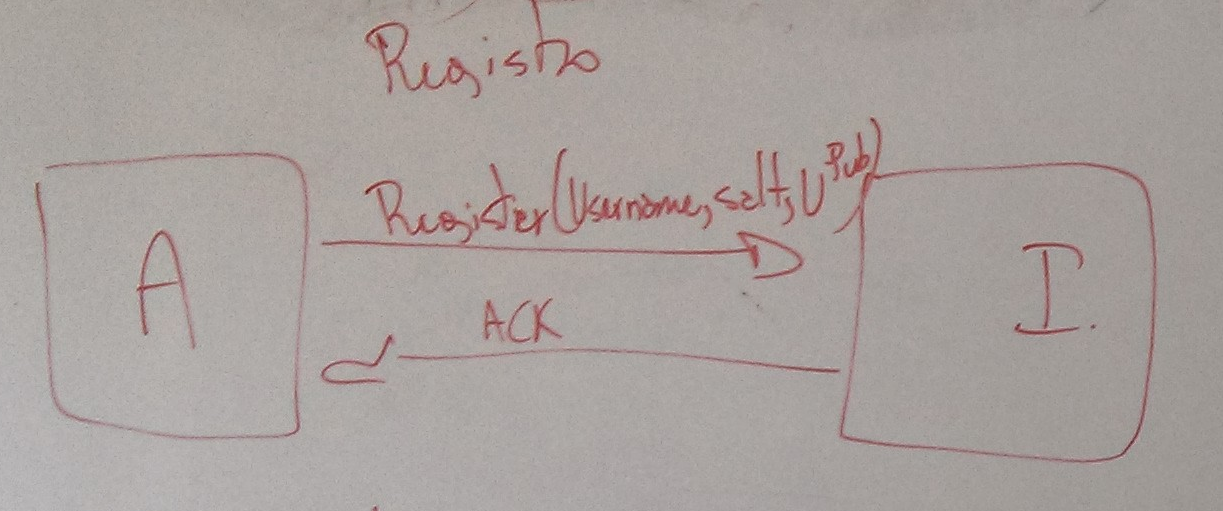
\includegraphics[width=14cm]{../img/registration_protocol_mockup.png}\\

\begin{figure}[!htb]
\centering
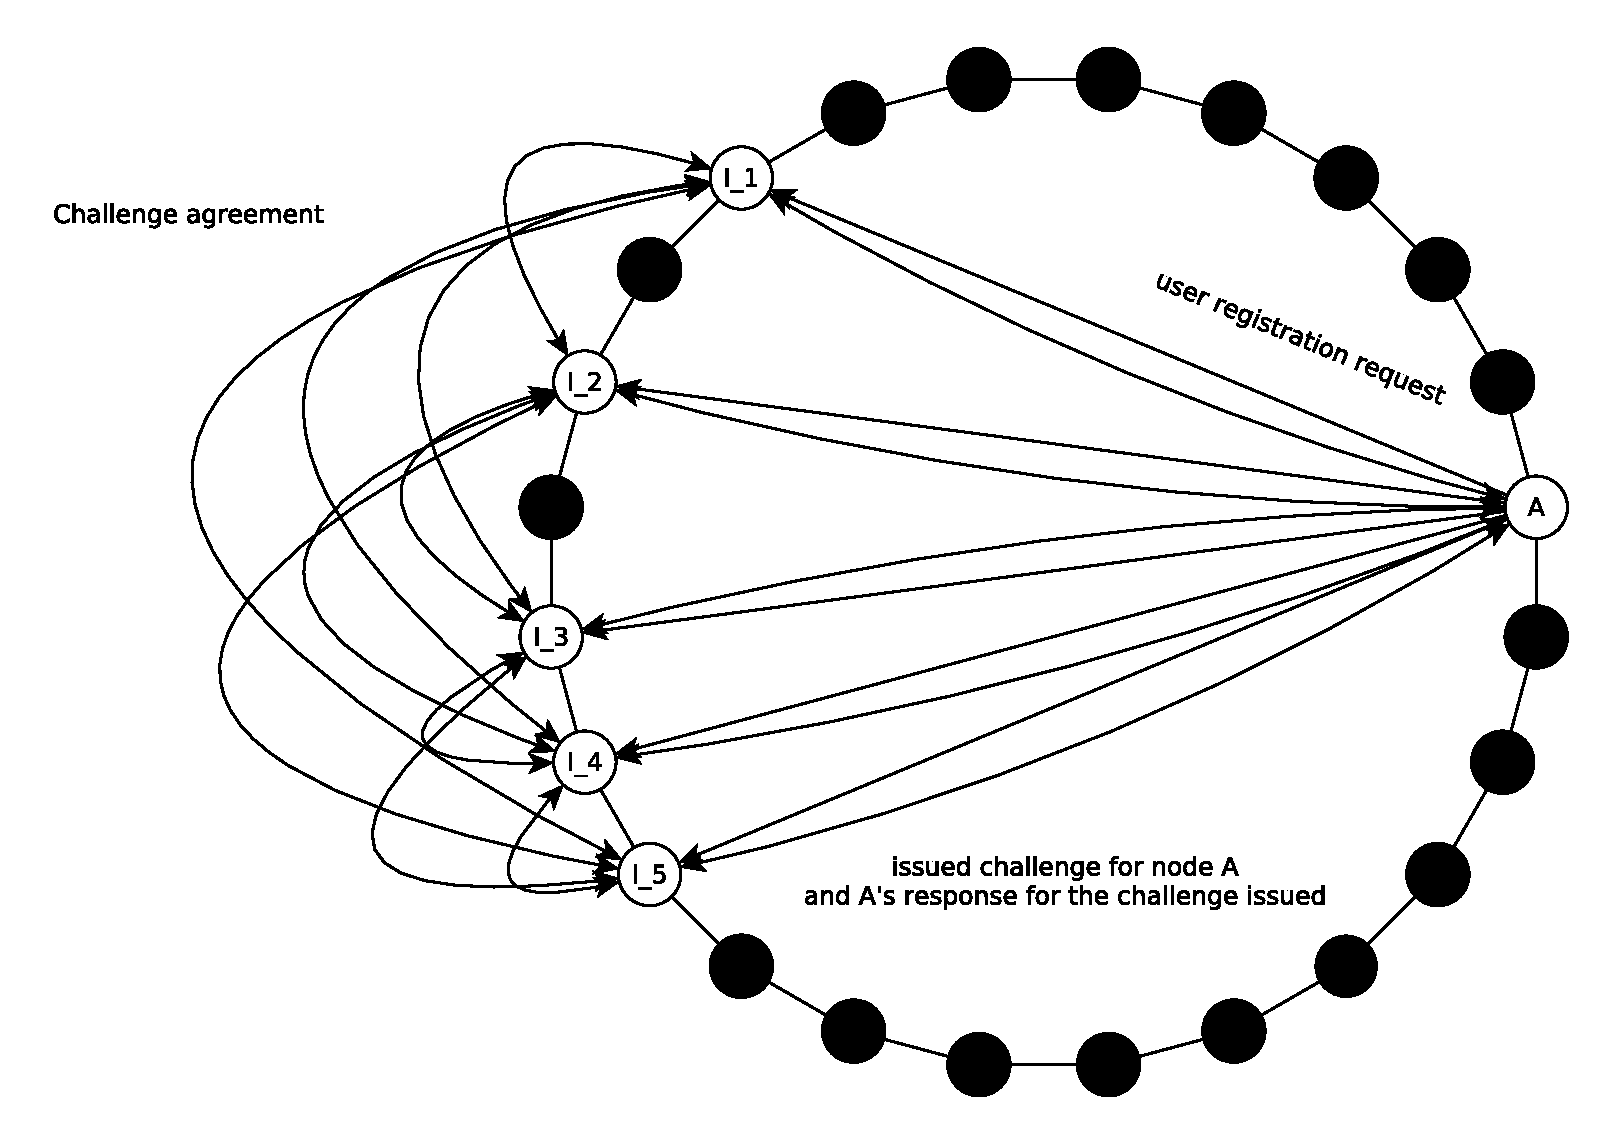
\includegraphics[width=14cm]{../img/sign_up}\\
\caption{Account registration.}
\label{fig:sign_up}
\end{figure}

To register a new user account ($U$), the node first
has to choose a \textit{username} and a \textit{password}.
%The \textit{username} should be unique in the network.
% The user checks if the username exists by sending a
% REGISTER(username, identity_file: [[c(user_keys_file), salt]).
% This operation use a accounted routing algorithm that uses only trusted
% nodes. When the register operation reaches the closest node to the username,
% it propagates a TRUSTSET_USERNAME_REGISTRATION operation. This operation sends a
% call to each node in the trustset of the node, which then pass to do a council
% meeting. If the meeting results in favor, each of them sends a
% OK_USERNAME_REGISTRATION(user_identity_file_name) to node doing the REGISTER operation.
% 
% DETAILS OF THE REGISTER OPERATION
% DETAILS OF THE COUNCIL MEETING --> Explain before, in trusted node part 
% 

% key store file
Then, a key derivation process is issued to generate the user private and
public keys. The
key derivation utilizes a \textit{salt} ($U^{salt}$) and a password ($U^{password}$) to
obtain the user's private and public Keys
($U^{priv}$ and $U^{pub}$).

The main idea behind the use of a \textit{salt} file is to avoid having a
situation where two users with the same password have the same private and
public keys.

The node  looks for the set $I$ set of nodes that will constitute the
identification service for the user $U$. To obtain the list of nodes that provides the user identification service for
the username $U^{username}$, the node $A$ computes its key $K$ such that $K =
SHA(U^{username})$. 

Then the node $A$ sends a request to every node $I_i$ in $I$ to register the
$U^{Pub}$ under the chosen  username  $U^{username}$.

%Then the node $A$ sends a request to every node $I_i$ in $I$ to register the
%$U^{salt}$ and $U^{Pub}$ under the chosen  username  $U^{username}$.

Each node in $I$ agrees in generating a random challenge~\ref{sec:challenges_puzzles}, which is then sent to the
client $A$ by every node $I_i \in I$ using the node public key to encrypt the
message.

If the node $A$ succeeds in answering correctly to the challenge, each node $I_i \in I$ then sends a user registration confirmation message to all nodes
in $I$ containing the new user public key. If a node $I_i$ receives at
%in $I$ containing the new user public key and salt. If a node $I_i$ receives at
least $\frac{L}{2} + 1$ identical user registration confirmation messages from
the others nodes in $I$, it sends a affirmative answer to the node $A$.

When the node
$A$ receives at least $\frac{L}{2} + 1$ identical affirmative answers from
$I$ regarding the user registration, then $A$ assumes that the user was
actually registered.

In~\ref{fig:sign_up} we show the process of a node $A$ doing an user account
registration with its identificator nodes $I_i \in I$.

%unique username
In case that the username was taken,
the node $A$ is prompted for a new username.



\subsection{User sign in}
%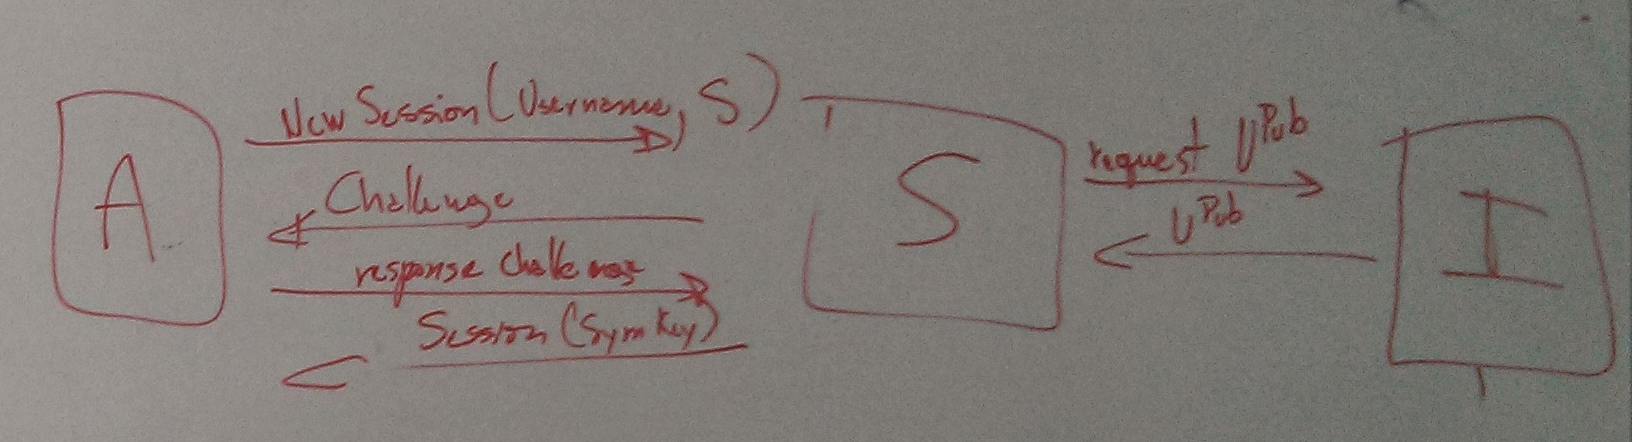
\includegraphics[width=14cm]{../img/session_creation_protocol_mockup}\\
\begin{figure}[!htb]
\centering
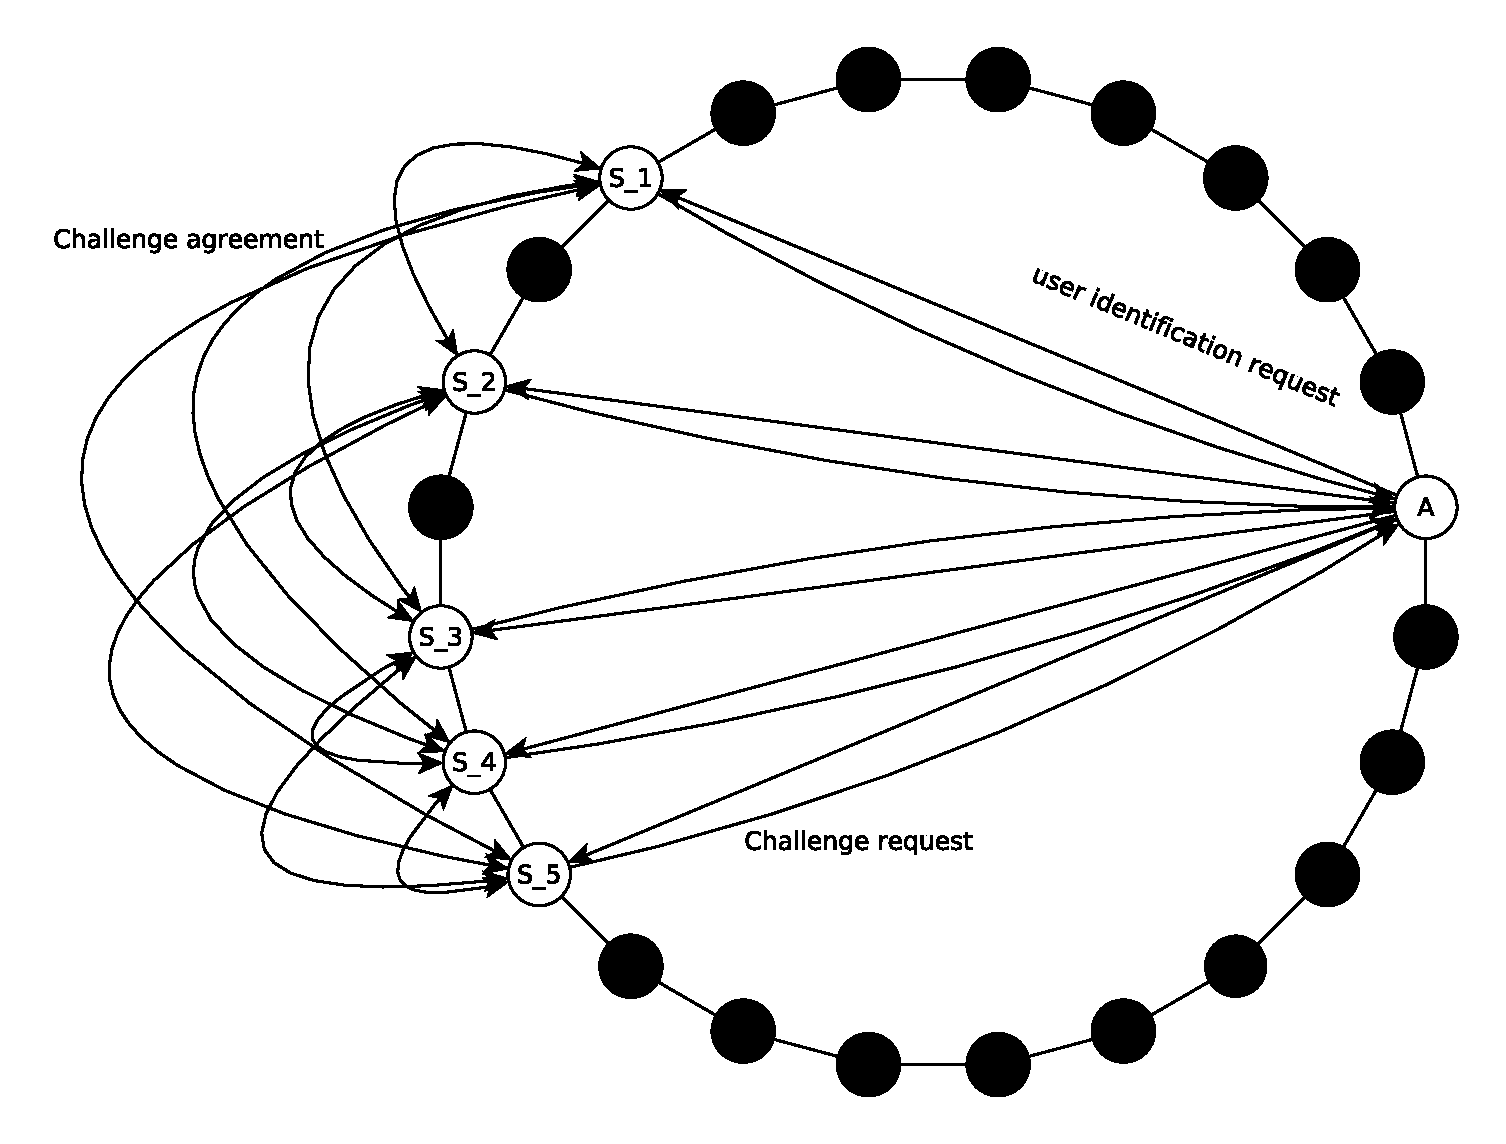
\includegraphics[width=14cm]{../img/sign_in}\\
\caption{User sign in: A service $S$ issues challenge to node $A$.}
\label{fig:sign_in}
\end{figure}

Before carrying out a transaction for a client $A$, a service $S$ proceeds to
verify the identity of the client from another set $I$ of nodes. At the end of
the identification process, the objective is to return a session key to $A$
and to store the created session on the nodes that belong $S$.

Each node $S_i \in S$ agrees in generating a random challenge~\ref{sec:challenges_puzzles}, which is then sent to the
client $A$ by every node $S_i \in S$ using the user public key to encrypt the
message.

Then, client $A$ responds each request with the corresponding answer to the
challenge encrypted with his user private key $U^{priv}$, generating
$E^{challenge}_{U^{priv}}$~\ref{fig:sign_in}. 

Upon reception of the $E^{secret_i}_{U^{priv}}$ message from the client $A$, every node in $S$
starts looking for the set $I$ of nodes that will constitute the quasi
identification authority. As seen in user identification service~\ref{sec:identificators}, to
determine which nodes belong to $I$, $S$ computes
its key $K$ such that $K = SHA(U^{username})$~\ref{fig:sign_in_2}.

\begin{figure}[!htb]
\centering
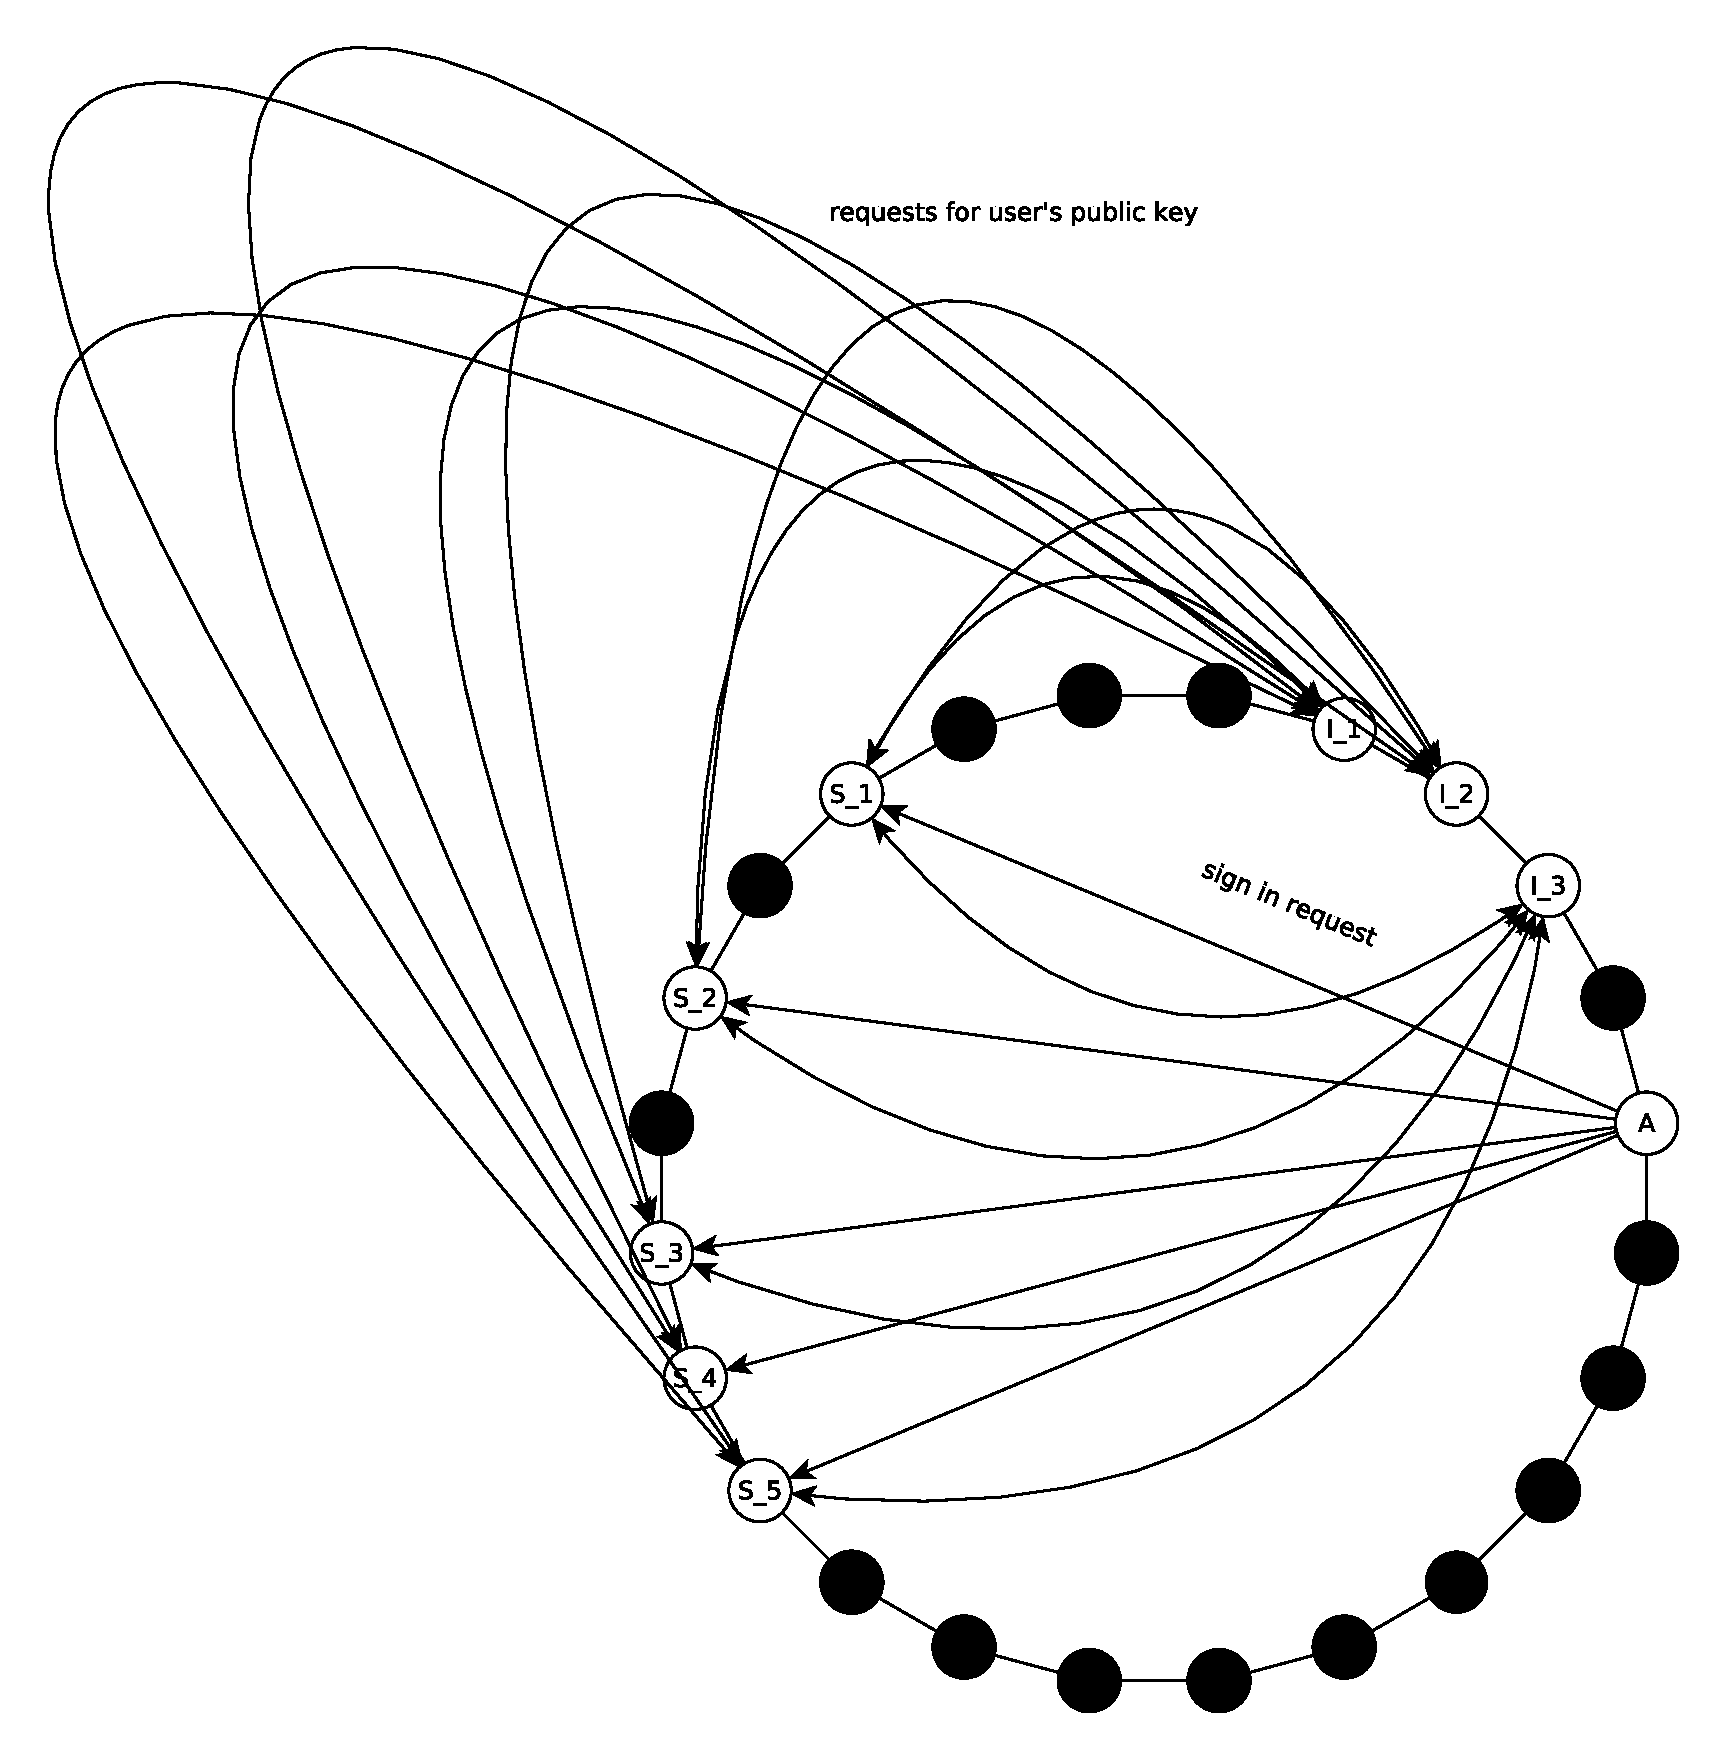
\includegraphics[width=14cm]{../img/sign_in_2}\\
\caption{User sign in: Nodes in $S$ requests the user's public key to the
identificators nodes of the user $U$.}
\label{fig:sign_in_2}
\end{figure}

Then each node in $S$ sends a request to every node $I_i$ in $I$ asking for the Username public key $U^{pub}$. When a node
$S_i$ of $S$ receives at least $\frac{L}{2} + 1$ identical answers from
$I$ regarding the $U^{pub}$, then $S_i$ assumes that the public key received
actually corresponds to the Username being identified. Each node $S_i$ in $S$
uses the $U^{pub}$ to decrypt $E^{secret_i}_{U^{priv}}$. If the result matches
the shared random secret $S^{secret}_i$, $S_i$ recognizes the node $A$ as the
user $U$.
Lastly, each node in $S$ agrees in the generation of the sessions keys for the
node $A$, which is then sent to the client $A$ by every node $S_i \in S$ using
the user public key to encrypt it. The session keys are stored in the
nodes that belong to $S$~\ref{fig:sign_in_3}.

\begin{figure}[!htb]
\centering
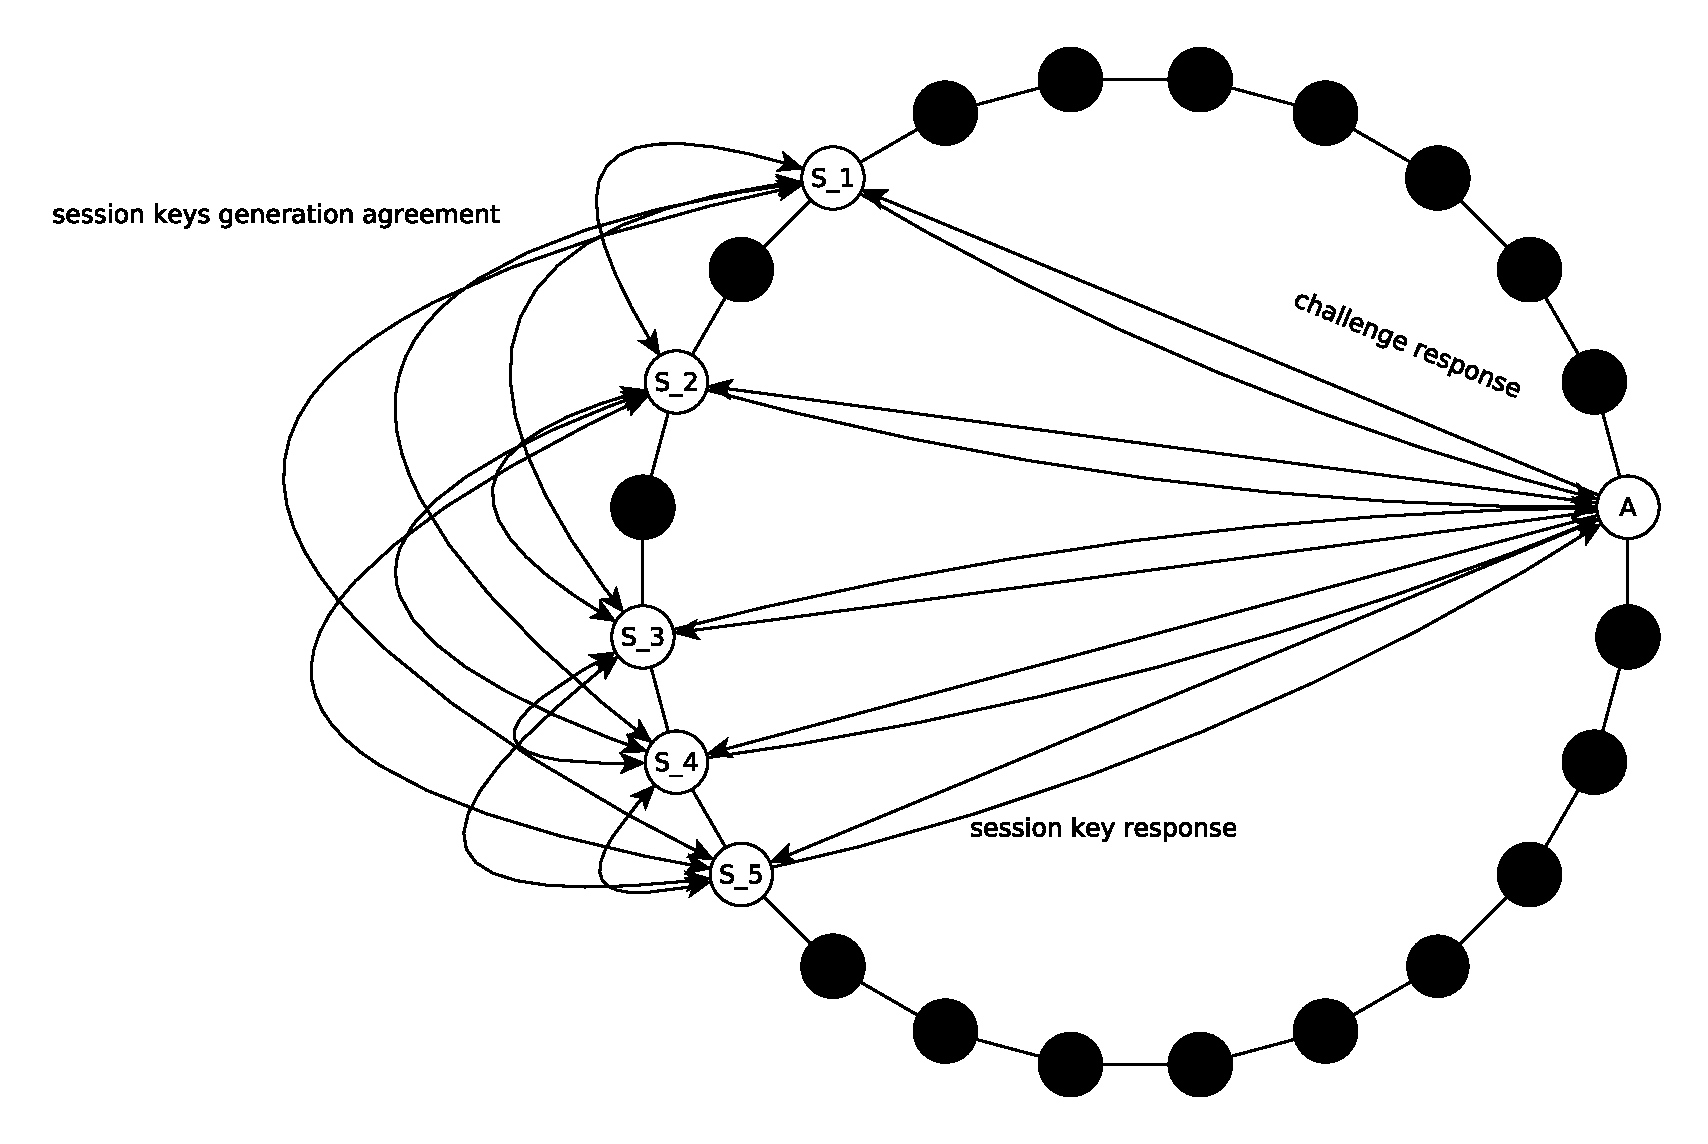
\includegraphics[width=14cm]{../img/sign_in_3}\\
\caption{User sign in: Nodes in $S$ generates the sessions keys for the node
$A$ identified as the user $U$.}
\label{fig:sign_in_3}
\end{figure}

\subsection{Logout}
The session are maintained by each service the user identified with. To close a
session, the node identified as the user $U$ sends a session close request to
the service $S$ using the session keys for the transaction. Also, the sessions
keys are issued for a certain time. After that time is passed, the node needs
to ask for a new session key with the service.


\subsection{Password Change}

First, the node $A$ needs to recover his actual private key using the process
in~\ref{sec:private_key_recovery}. Then the node $A$ generates a new private/public
key pair using the new password.  With this, the node $A$ request a
password change to every node $I_i$ in $I$. The request is signed with the
actual user private keys, and includes the new user public key $U^{pub}_{new}$.
%and salt used to derive his new private key $U^{salt}_{new}$. 
Each node $I_i \in I$ then sends a password change confirmation message to all nodes
in $I$ containing the new user public key. If a node $I_i$ receives at
least $\frac{L}{2} + 1$ identical password change confirmation messages from
the others nodes in $I$, it sends a affirmative answer to the node $A$.
 When the node $A$ receives at least $\frac{L}{2} + 1$ identical affirmative
answers from $I$ regarding the user password change, then $A$ assumes that the
user keys (and password) were updated.

\subsection{User private key recovery (Discarded protocol)}
\label{sec:private_key_recovery}
%\includegraphics[width=14cm]{../img/sign in_protocol_mockup}\\
\paragraph{Why was discarded?}
This protocol was discarded because it offers a weak security for the user's
private keys, which are used to identify the user in the system.  While the main idea
of this protocol is to let users sign in without the need to
manage a copy of the user's private key, it is prone to offline attacks. In
offline attacks, a malicious user tries different password to generate the
public and private key till getting the same that is published in the network
for an specific user.

\paragraph{Protocol A}

First, the node $A$ looks for the set $I$ of nodes that will constitute the
identification service for the user $U$.
To obtain the list of nodes $I$ that provides the user identification service for
the username $U^{username}$, the node $A$ computes its key $K$ such that $K =
SHA(U^{username})$. 
Then the node $A$ sends a request to every node $I_i$ in $I$ to obtain the user
salt $U^{salt}$ needed to derive the user private key $U^{priv}$.
 When the node $A$ receives at least $\frac{L}{2} + 1$ identical affirmative answers from
$I$ regarding the user salt, then $A$ assumes that the salt retrieved
corresponds to the one registered previously by the user ($U^{salt}$). Finally,
the node proceeds to derive the user private key $U^{priv}$ using his user password $U^{password}$.


\subsubsection{Changes to the other protocols}
\paragraph{User registration}
The node $A$ needs to also register the \textit{salt} $U^{salt}$ used to
generate its private key. This is stored alongside the user's public keys $U^{Pub}$ under the
chosen username $U^{username}$.

%Then the node $A$ sends a request to every node $I_i$ in $I$ to register the
%$U^{salt}$ and $U^{Pub}$ under the chosen  username  $U^{username}$.

\paragraph{Password Change}
When re-registering the user's public key, the node $A$ needs to also register the \textit{salt} $U^{salt}$ used to
re-generate its private key. This is stored alongside the new user's public keys $U^{Pub}$ under the
chosen username $U^{username}$.

%actual user private keys, and includes the new user public key $U^{pub}_{new}$
%and salt used to derive his new private key $U^{salt}_{new}$. 

\paragraph{Protocol B}

This protocol use indirection and anonymity layers to hide the user's
\textit{salt} and obscure their whereabouts in the storage service.
To made this possible, we mount another storage service called secret storage
on top of the storage service used in the P2P network. The secret storage is conformed
by the same nodes that serve the storage system for the DHT, but the function
used to route a keyword to a node differs. The main idea of the secret storage
is to put the user's \textit{salt} used to generate his private keys in a
path only known for him. The function used to know in what node the
\textit{salt} will be stored is $SHA(SHA(username)+SHA(password))$, and the
filename of the stored \textit{salt} will be
$SHA(SHA(password)+SHA(username))$. The secret storage is of public access for
the network, and is used to recreate the user's private key using the user's
\textit{salt} and the user's password. Also, to obfuscate the node identity that
stored the file, the query to store it uses the onion network route protocol to
send it.

%Then, when the user needs to recover his private key, the system uses his
%username and password to know where is stored and how is the filename that
%needs to retrieve.  First, the node $A$ looks for the nodes forming the secret storage ($SS$) set of nodes that will constitute the
%identification service for the user $U$.
%To obtain the list of nodes $I$ that provides the user identification service for
%the username $U^{username}$, the node $A$ computes its key $K$ such that $K =
%SHA(U^{username})$. 
%Then the node $A$ sends a request to every node $I_i$ in $I$ to obtain the user
%salt $U^{salt}$ needed to derive the user private key $U^{priv}$.
% When the node $A$ receives at least $\frac{L}{2} + 1$ identical affirmative answers from
%$I$ regarding the user salt, then $A$ assumes that the salt retrieved
%corresponds to the one registered previously by the user ($U^{salt}$). Finally,
%the node proceeds to derive the user private key $U^{priv}$ using his user password $U^{password}$.
